\chapter{Эксперимент 4: Исследование способов эффективного чтения оперативной памяти}

\section{Цель эксперимента}
Исследовать возможности ускорения вычислений благодаря использованию структур данных, оптимизирующих механизм чтения оперативной памяти. 

\section{Описание проблемы}
При  обработке информации, находящейся в нескольких страницах и банках оперативной памяти возникают задержки, связанные с необходимостью открытия и закрытия страниц DRAM памяти. При программировании на языках высокого уровня такая ситуация наблюдается при интенсивной обработки нескольких массивов данных или обработке многомерных массивов. При этом процессоры, в которых реализованы механизмы аппаратной предвыборки, часто не могут организовать эффективную загрузку данных. Кроме этого, объемы запрошенных данных оказываются заметно меньше размера пакета, передаваемого из оперативной памяти. Таким образом, эффективная обработка нескольких векторных структур данных без их дополнительной оптимизации не использует в должной степени возможности аппаратных ресурсов. 

\section{Суть эксперимента}
Для сравнения производительности алгоритмов, использующих оптимизированные и неоптимизированные структуры данных используется профилировка кода двух подпрограмм, каждая из которых должна выполнить обработку нескольких блоков оперативной памяти. В алгоритмах обрабатываются двойные слова данных (4 байта), что существенно меньше размера пакета (32 - 128 байт). Неоптимизированный вариант структуры данных представляет собой несколько массивов в оперативной памяти, в то время как оптимизированная структура состоит из чередующихся данных каждого массива.

\section{Условия эксперимента}
\begin{enumerate}
    \item Единицы измерения по Ох - Колличество параллельных потоков;
    \item Единицы измерения по Оу - Такты;
    \item Размер массива: \textbf{2};
    \item Количество потоков данных: \textbf{64};
\end{enumerate}

\section{Результаты эксперимента}
\begin{figure}[ht!]
    \centering
    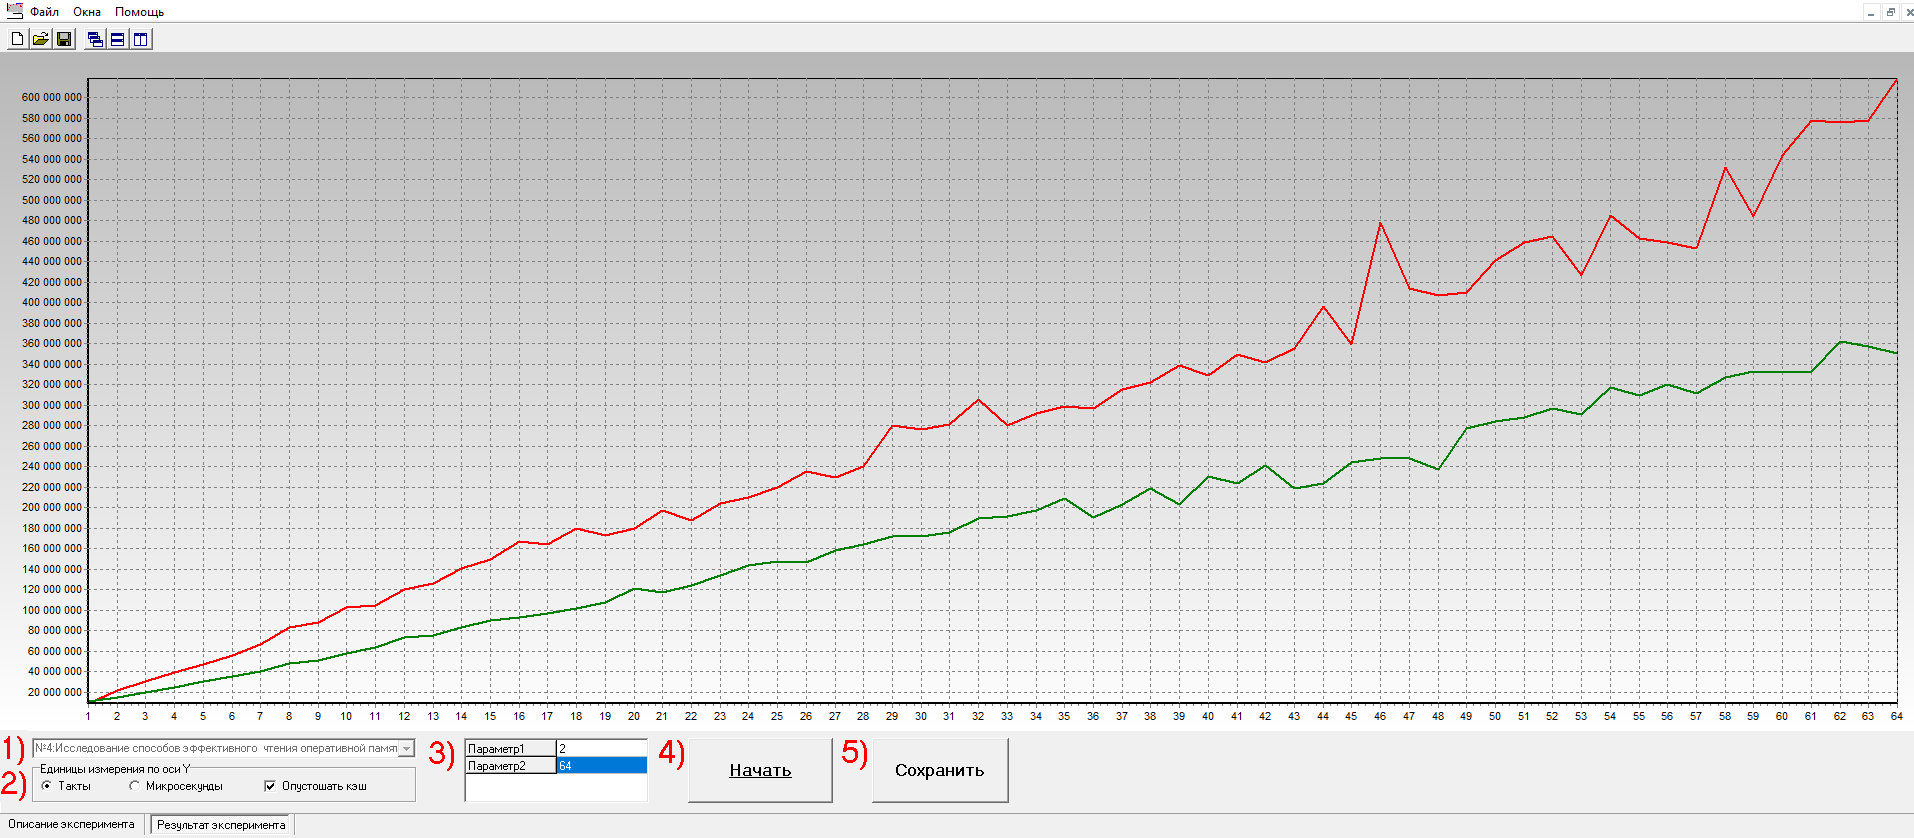
\includegraphics[width=170mm]{./img/4.png}
    \caption{Эксперимент 4: Исследование способов эффективного чтения оперативной памяти}
\end{figure}

\begin{figure}[ht!]
    \centering
    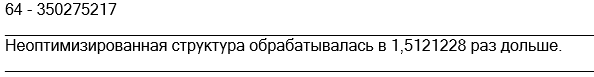
\includegraphics[width=100mm]{./img/04.png}
    \caption{Эксперимент 4: Результаты\label{res_04}}
\end{figure}

Как видно на рисунке \ref{res_04}, неоптимизированная структура обрабатывалась примерно в 1,5 раз дольше.

\section{Вывод}
Исходя из полученных результатов, можно сделать вывод, что упорядоченные данные могут позволить ускорить работу алгоритма.